\documentclass[11pt,a4paper]{article}



% abstract
\def\abstract{%
    \quotation\small }
\def\endabstract{\vspace{1.6em}\par\endquotation
    \normalsize\rm}

	

\linespread{1.3}
\usepackage{geometry}
\geometry{top=1in, bottom=1in,left=1in,right=1in}

\usepackage{fancyhdr}
\pagestyle{fancy}
\lhead{}
\chead{无透镜傅里叶全息显微}
\rhead{左元 SA13006060}
\lfoot{}
\cfoot{\thepage}
\rfoot{}
\renewcommand{\headrulewidth}{0.4pt}
\renewcommand{\footrulewidth}{0.4pt}


\usepackage{amsmath}

\usepackage{xeCJK}
\setCJKmainfont{SimSun}

\bibliographystyle{IEEEtran}

\newcommand{\half}{\frac{1}{2}}	% 1/2
\renewcommand{\figurename}{图}
\renewcommand{\tablename}{表}

\title{无透镜傅里叶全息显微}
\author{左元 SA13006060}
\date{\today}


\begin{document}

\maketitle

\begin{abstract}
\noindent
\textbf{摘要:}数字全息技术是光学成像领域一项新兴技术,
而数字全息显微技术则是应用这种方法实现显微成像的。
在本文中,我首先回顾一下数字全息显微技术的背景,
接着推导一下成像的理论,并根据理论进行数值仿真,
验证理论的正确性。
\end{abstract}

\section{简介}
为了提高电子显微镜的分辨能力,Dennis Gabor发明于1948年被全息术。
他意识到电子束的衍射图样包含了物象的所有信息,
因此,通过记录衍射场,可以重建目标的物场。
因为这种方法可以记录整个光场,所以他称之为全息术(holography)\cite{gabor1948new, kim2010principles}。

全息术马上被应用到可见光成像领域,
但是直到两项关键技术的出现,它的潜能才被完全挖掘出来。
这两项关键技术分别是激光器为代表的理想的相干光源,
还有就是Leith和Upatnieks发明的分立参考光离轴照明技术\cite{leith1962reconstructed}。
这种照明方式解决了Gabor装置中,重建过程中实像、0级干涉像和共轭像的分离。
之后,全息术的应用得到飞速发展,到现在已是一个成熟的领域了。

对于很多领域的应用来说,实现实时的处理是非常有用的,
但是用传统实现全息的方式却非常难。
数字全息术通过利用电子设备代替物理和化学的记录方式,
利用数值计算模拟光学重建过程,很好的解决了这一问题。
光场传播可以通过衍射理论进行精确地描述,
在1967年,Goodman和Lawrence从摄像机中得到的傅里叶全息图中,
通过数值重建的方法证实了数值重建的可行性\cite{goodman1967digital}。
而在1994年,德国科学家Schnars和Jueptner采用离轴菲涅尔全息记录光路,
用CCD记录了一个骰子的全息图,并重建出了清晰的物场图像\cite{schnars1994direct}。

数字全息显微是通过数字全息术实现显微成像的技术。
它被广泛应用到生命科学、医学等领域,
国际上数字全息显微成像的分辨率已经达到横向亚微米量级、轴向纳米量级\cite{kemper2008digital,marquet2005digital,mann2006quantitative}。
近年来,数字全息显微成像开始考虑向廉价的实现发展,
通过无透镜傅里叶全息光路,可以在手机上通过增加少量的外设实现\cite{breslauer2009mobile,tseng2010lensfree,vashist2014cellphone}。
采用这种方式,将有可能让数字全息显微的技术走向每个家庭。

\section{数字全息成像的理论分析}
数字全息成像的基本原理与普通光学全息成像是相同的,
成像的过程分为两步:首先通过物光和参考光干涉形成干涉图样,将干涉图样记录下来;
然后用另一参考光去照明记录下的干涉图样,就可以重建物光场。
与普通全息成像用胶片等物理和化学方法记录干涉图样所不同的是,
数字全息成像利用CCD相机记录干涉图样的采样值,如图\ref{fig:dh}所示,
而且数字全息成像重建过程都是通过计算机软件实现的。

\begin{figure}[htb]
  \centering
  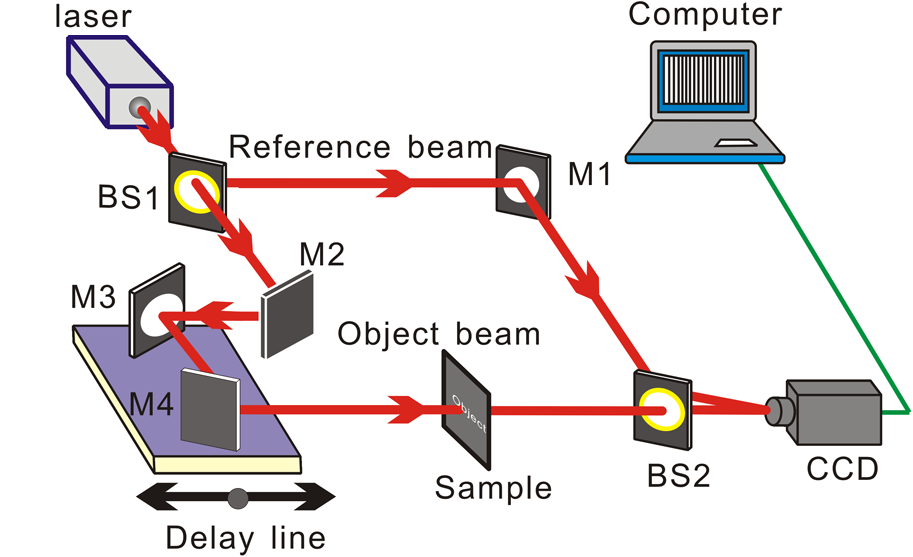
\includegraphics[width=0.8\textwidth]{fig1.png}
  \caption{数字全系成像示意图}
  \label{fig:dh}
\end{figure}

从目标处反射或透射的光到达CCD的过程,可以通过衍射理论来描述。
如图\ref{fig:diffraction}所示,设目标物反射或投射的光场在$\Sigma_0$平面处为$E_0(x_0,y_0)$,
其中$(x_0, y_0)$是$\Sigma_0$平面的坐标,那么利用惠更斯-菲涅尔原理,到达成像平面$\Sigma$的光场为
\begin{equation}
E(x, y; z) = - \frac{i k}{2 \pi z} \iint_{\Sigma_0} dx_0 dy_0 E_0(x_0,y_0) \exp(i k \sqrt{(x-x_0)^2+(y-y_0)^2+z^2})
\label{eq:huygens}
\end{equation}
其中$k=\frac{2 \pi}{\lambda}$为波数,$z$ 是物平面和像平面间的距离。
上式也可以表达为卷积形式
\begin{equation}
E(x,y; z) = E_0(x , y) \ast S_H(x, y; z)
\end{equation}
式中点扩展函数(PSF) $S_H$代表惠更斯球面波,
\begin{equation}
S_H(x, y; z) =  - \frac{i k}{2 \pi z} \exp(i k \sqrt{(x-x_0)^2+(y-y_0)^2+z^2})
\end{equation}
式(\ref{eq:huygens})表示像平面的光场是由物场所有点源发出的球面波的叠加。

\begin{figure}[htb]
  \centering
  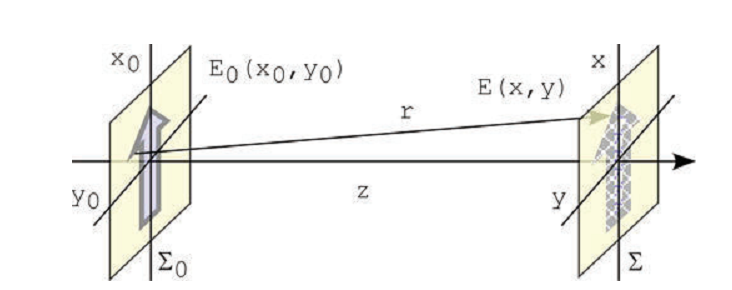
\includegraphics[width=0.8\textwidth]{diffraction.png}
  \caption{衍射过程的示意图}
  \label{fig:diffraction}
\end{figure}

\section{无透镜傅里叶全息显微}

\section{总结}


\bibliographystyle{IEEEtran}
\bibliography{ref}

\end{document}